% Options for packages loaded elsewhere
\PassOptionsToPackage{unicode}{hyperref}
\PassOptionsToPackage{hyphens}{url}
\PassOptionsToPackage{dvipsnames,svgnames,x11names}{xcolor}
%
\documentclass[
  letterpaper,
  DIV=11,
  numbers=noendperiod]{scrreprt}

\usepackage{amsmath,amssymb}
\usepackage{iftex}
\ifPDFTeX
  \usepackage[T1]{fontenc}
  \usepackage[utf8]{inputenc}
  \usepackage{textcomp} % provide euro and other symbols
\else % if luatex or xetex
  \usepackage{unicode-math}
  \defaultfontfeatures{Scale=MatchLowercase}
  \defaultfontfeatures[\rmfamily]{Ligatures=TeX,Scale=1}
\fi
\usepackage{lmodern}
\ifPDFTeX\else  
    % xetex/luatex font selection
    \setmainfont[]{Noto Sans KR}
\fi
% Use upquote if available, for straight quotes in verbatim environments
\IfFileExists{upquote.sty}{\usepackage{upquote}}{}
\IfFileExists{microtype.sty}{% use microtype if available
  \usepackage[]{microtype}
  \UseMicrotypeSet[protrusion]{basicmath} % disable protrusion for tt fonts
}{}
\makeatletter
\@ifundefined{KOMAClassName}{% if non-KOMA class
  \IfFileExists{parskip.sty}{%
    \usepackage{parskip}
  }{% else
    \setlength{\parindent}{0pt}
    \setlength{\parskip}{6pt plus 2pt minus 1pt}}
}{% if KOMA class
  \KOMAoptions{parskip=half}}
\makeatother
\usepackage{xcolor}
\setlength{\emergencystretch}{3em} % prevent overfull lines
\setcounter{secnumdepth}{5}
% Make \paragraph and \subparagraph free-standing
\makeatletter
\ifx\paragraph\undefined\else
  \let\oldparagraph\paragraph
  \renewcommand{\paragraph}{
    \@ifstar
      \xxxParagraphStar
      \xxxParagraphNoStar
  }
  \newcommand{\xxxParagraphStar}[1]{\oldparagraph*{#1}\mbox{}}
  \newcommand{\xxxParagraphNoStar}[1]{\oldparagraph{#1}\mbox{}}
\fi
\ifx\subparagraph\undefined\else
  \let\oldsubparagraph\subparagraph
  \renewcommand{\subparagraph}{
    \@ifstar
      \xxxSubParagraphStar
      \xxxSubParagraphNoStar
  }
  \newcommand{\xxxSubParagraphStar}[1]{\oldsubparagraph*{#1}\mbox{}}
  \newcommand{\xxxSubParagraphNoStar}[1]{\oldsubparagraph{#1}\mbox{}}
\fi
\makeatother

\usepackage{color}
\usepackage{fancyvrb}
\newcommand{\VerbBar}{|}
\newcommand{\VERB}{\Verb[commandchars=\\\{\}]}
\DefineVerbatimEnvironment{Highlighting}{Verbatim}{commandchars=\\\{\}}
% Add ',fontsize=\small' for more characters per line
\usepackage{framed}
\definecolor{shadecolor}{RGB}{241,243,245}
\newenvironment{Shaded}{\begin{snugshade}}{\end{snugshade}}
\newcommand{\AlertTok}[1]{\textcolor[rgb]{0.68,0.00,0.00}{#1}}
\newcommand{\AnnotationTok}[1]{\textcolor[rgb]{0.37,0.37,0.37}{#1}}
\newcommand{\AttributeTok}[1]{\textcolor[rgb]{0.40,0.45,0.13}{#1}}
\newcommand{\BaseNTok}[1]{\textcolor[rgb]{0.68,0.00,0.00}{#1}}
\newcommand{\BuiltInTok}[1]{\textcolor[rgb]{0.00,0.23,0.31}{#1}}
\newcommand{\CharTok}[1]{\textcolor[rgb]{0.13,0.47,0.30}{#1}}
\newcommand{\CommentTok}[1]{\textcolor[rgb]{0.37,0.37,0.37}{#1}}
\newcommand{\CommentVarTok}[1]{\textcolor[rgb]{0.37,0.37,0.37}{\textit{#1}}}
\newcommand{\ConstantTok}[1]{\textcolor[rgb]{0.56,0.35,0.01}{#1}}
\newcommand{\ControlFlowTok}[1]{\textcolor[rgb]{0.00,0.23,0.31}{\textbf{#1}}}
\newcommand{\DataTypeTok}[1]{\textcolor[rgb]{0.68,0.00,0.00}{#1}}
\newcommand{\DecValTok}[1]{\textcolor[rgb]{0.68,0.00,0.00}{#1}}
\newcommand{\DocumentationTok}[1]{\textcolor[rgb]{0.37,0.37,0.37}{\textit{#1}}}
\newcommand{\ErrorTok}[1]{\textcolor[rgb]{0.68,0.00,0.00}{#1}}
\newcommand{\ExtensionTok}[1]{\textcolor[rgb]{0.00,0.23,0.31}{#1}}
\newcommand{\FloatTok}[1]{\textcolor[rgb]{0.68,0.00,0.00}{#1}}
\newcommand{\FunctionTok}[1]{\textcolor[rgb]{0.28,0.35,0.67}{#1}}
\newcommand{\ImportTok}[1]{\textcolor[rgb]{0.00,0.46,0.62}{#1}}
\newcommand{\InformationTok}[1]{\textcolor[rgb]{0.37,0.37,0.37}{#1}}
\newcommand{\KeywordTok}[1]{\textcolor[rgb]{0.00,0.23,0.31}{\textbf{#1}}}
\newcommand{\NormalTok}[1]{\textcolor[rgb]{0.00,0.23,0.31}{#1}}
\newcommand{\OperatorTok}[1]{\textcolor[rgb]{0.37,0.37,0.37}{#1}}
\newcommand{\OtherTok}[1]{\textcolor[rgb]{0.00,0.23,0.31}{#1}}
\newcommand{\PreprocessorTok}[1]{\textcolor[rgb]{0.68,0.00,0.00}{#1}}
\newcommand{\RegionMarkerTok}[1]{\textcolor[rgb]{0.00,0.23,0.31}{#1}}
\newcommand{\SpecialCharTok}[1]{\textcolor[rgb]{0.37,0.37,0.37}{#1}}
\newcommand{\SpecialStringTok}[1]{\textcolor[rgb]{0.13,0.47,0.30}{#1}}
\newcommand{\StringTok}[1]{\textcolor[rgb]{0.13,0.47,0.30}{#1}}
\newcommand{\VariableTok}[1]{\textcolor[rgb]{0.07,0.07,0.07}{#1}}
\newcommand{\VerbatimStringTok}[1]{\textcolor[rgb]{0.13,0.47,0.30}{#1}}
\newcommand{\WarningTok}[1]{\textcolor[rgb]{0.37,0.37,0.37}{\textit{#1}}}

\providecommand{\tightlist}{%
  \setlength{\itemsep}{0pt}\setlength{\parskip}{0pt}}\usepackage{longtable,booktabs,array}
\usepackage{calc} % for calculating minipage widths
% Correct order of tables after \paragraph or \subparagraph
\usepackage{etoolbox}
\makeatletter
\patchcmd\longtable{\par}{\if@noskipsec\mbox{}\fi\par}{}{}
\makeatother
% Allow footnotes in longtable head/foot
\IfFileExists{footnotehyper.sty}{\usepackage{footnotehyper}}{\usepackage{footnote}}
\makesavenoteenv{longtable}
\usepackage{graphicx}
\makeatletter
\def\maxwidth{\ifdim\Gin@nat@width>\linewidth\linewidth\else\Gin@nat@width\fi}
\def\maxheight{\ifdim\Gin@nat@height>\textheight\textheight\else\Gin@nat@height\fi}
\makeatother
% Scale images if necessary, so that they will not overflow the page
% margins by default, and it is still possible to overwrite the defaults
% using explicit options in \includegraphics[width, height, ...]{}
\setkeys{Gin}{width=\maxwidth,height=\maxheight,keepaspectratio}
% Set default figure placement to htbp
\makeatletter
\def\fps@figure{htbp}
\makeatother
% definitions for citeproc citations
\NewDocumentCommand\citeproctext{}{}
\NewDocumentCommand\citeproc{mm}{%
  \begingroup\def\citeproctext{#2}\cite{#1}\endgroup}
\makeatletter
 % allow citations to break across lines
 \let\@cite@ofmt\@firstofone
 % avoid brackets around text for \cite:
 \def\@biblabel#1{}
 \def\@cite#1#2{{#1\if@tempswa , #2\fi}}
\makeatother
\newlength{\cslhangindent}
\setlength{\cslhangindent}{1.5em}
\newlength{\csllabelwidth}
\setlength{\csllabelwidth}{3em}
\newenvironment{CSLReferences}[2] % #1 hanging-indent, #2 entry-spacing
 {\begin{list}{}{%
  \setlength{\itemindent}{0pt}
  \setlength{\leftmargin}{0pt}
  \setlength{\parsep}{0pt}
  % turn on hanging indent if param 1 is 1
  \ifodd #1
   \setlength{\leftmargin}{\cslhangindent}
   \setlength{\itemindent}{-1\cslhangindent}
  \fi
  % set entry spacing
  \setlength{\itemsep}{#2\baselineskip}}}
 {\end{list}}
\usepackage{calc}
\newcommand{\CSLBlock}[1]{\hfill\break\parbox[t]{\linewidth}{\strut\ignorespaces#1\strut}}
\newcommand{\CSLLeftMargin}[1]{\parbox[t]{\csllabelwidth}{\strut#1\strut}}
\newcommand{\CSLRightInline}[1]{\parbox[t]{\linewidth - \csllabelwidth}{\strut#1\strut}}
\newcommand{\CSLIndent}[1]{\hspace{\cslhangindent}#1}

\usepackage{makeidx}
\makeindex
\usepackage{titling}
\usepackage{pdfpages}
\usepackage{atbegshi}% http://ctan.org/pkg/atbegshi
\usepackage{kotex}
\let\oldmaketitle\maketitle
\AtBeginDocument{\let\maketitle\relax}
\AtBeginDocument{\AtBeginShipoutNext{\AtBeginShipoutDiscard}} % Discard next blank page





\KOMAoption{captions}{tableheading}
\makeatletter
\@ifpackageloaded{bookmark}{}{\usepackage{bookmark}}
\makeatother
\makeatletter
\@ifpackageloaded{caption}{}{\usepackage{caption}}
\AtBeginDocument{%
\ifdefined\contentsname
  \renewcommand*\contentsname{Table of contents}
\else
  \newcommand\contentsname{Table of contents}
\fi
\ifdefined\listfigurename
  \renewcommand*\listfigurename{List of Figures}
\else
  \newcommand\listfigurename{List of Figures}
\fi
\ifdefined\listtablename
  \renewcommand*\listtablename{List of Tables}
\else
  \newcommand\listtablename{List of Tables}
\fi
\ifdefined\figurename
  \renewcommand*\figurename{Figure}
\else
  \newcommand\figurename{Figure}
\fi
\ifdefined\tablename
  \renewcommand*\tablename{Table}
\else
  \newcommand\tablename{Table}
\fi
}
\@ifpackageloaded{float}{}{\usepackage{float}}
\floatstyle{ruled}
\@ifundefined{c@chapter}{\newfloat{codelisting}{h}{lop}}{\newfloat{codelisting}{h}{lop}[chapter]}
\floatname{codelisting}{Listing}
\newcommand*\listoflistings{\listof{codelisting}{List of Listings}}
\usepackage{amsthm}
\theoremstyle{definition}
\newtheorem{definition}{Definition}[chapter]
\theoremstyle{plain}
\newtheorem{theorem}{Theorem}[chapter]
\theoremstyle{definition}
\newtheorem{example}{Example}[chapter]
\theoremstyle{definition}
\newtheorem{exercise}{Exercise}[chapter]
\theoremstyle{remark}
\AtBeginDocument{\renewcommand*{\proofname}{Proof}}
\newtheorem*{remark}{Remark}
\newtheorem*{solution}{Solution}
\newtheorem{refremark}{Remark}[chapter]
\newtheorem{refsolution}{Solution}[chapter]
\makeatother
\makeatletter
\makeatother
\makeatletter
\@ifpackageloaded{caption}{}{\usepackage{caption}}
\@ifpackageloaded{subcaption}{}{\usepackage{subcaption}}
\makeatother
\makeatletter
\@ifpackageloaded{algorithm}{}{\usepackage{algorithm}}
\makeatother
\makeatletter
\@ifpackageloaded{algpseudocode}{}{\usepackage{algpseudocode}}
\makeatother
\makeatletter
\@ifpackageloaded{fontspec}{}{\usepackage{fontspec}}
\makeatother
\makeatletter
\@ifpackageloaded{draftwatermark}{}{\usepackage{draftwatermark}}
\makeatother
\makeatletter
\@ifpackageloaded{xcolor}{}{\usepackage{xcolor}}
\makeatother
\makeatletter
\@ifpackageloaded{forloop}{}{\usepackage{forloop}}
\makeatother
    \definecolor{watermark}{HTML}{000000}
    
    \newcounter{watermarkrow}
    \newcounter{watermarkcol}

    \DraftwatermarkOptions{
      text={
        \begin{tabular}{c}
          \forloop{watermarkrow}{0}{\value{watermarkrow} < 50}{
            \forloop{watermarkcol}{0}{\value{watermarkcol} < 10}{
              { Seoncheol\ Park}\hspace{4.000000em}
            }
            \\[4.000000em]
          }
        \end{tabular}
      },
      fontsize=1.000000em,
      angle=15.000000,
      color=watermark!10
    }
    
\ifLuaTeX
  \usepackage{selnolig}  % disable illegal ligatures
\fi
\usepackage{bookmark}

\IfFileExists{xurl.sty}{\usepackage{xurl}}{} % add URL line breaks if available
\urlstyle{same} % disable monospaced font for URLs
\hypersetup{
  pdftitle={A Biggner's Guide to Linear Models},
  pdfauthor={Seoncheol Park},
  colorlinks=true,
  linkcolor={blue},
  filecolor={Maroon},
  citecolor={Blue},
  urlcolor={Blue},
  pdfcreator={LaTeX via pandoc}}

\title{A Biggner's Guide to Linear Models}
\author{Seoncheol Park}
\date{2024-07-14}

\begin{document}
\maketitle

\renewcommand{\Return}{\State \textbf{return}~}
\newcommand{\Print}{\State \textbf{print}~}
\newcommand{\Break}{\State \textbf{break}}
\newcommand{\Continue}{\State \textbf{continue}}
\newcommand{\True}{\textbf{true}}
\newcommand{\False}{\textbf{false}}
\renewcommand{\And}{\textbf{and}~}
\newcommand{\Or}{\textbf{or}~}
\renewcommand{\Not}{\textbf{not}~}
\newcommand{\To}{\textbf{to}~}
\newcommand{\DownTo}{\textbf{downto}~}

\floatname{algorithm}{Algorithm}

\renewcommand*\contentsname{Table of contents}
{
\hypersetup{linkcolor=}
\setcounter{tocdepth}{2}
\tableofcontents
}
\bookmarksetup{startatroot}

\chapter*{Preface}\label{preface}
\addcontentsline{toc}{chapter}{Preface}

\markboth{Preface}{Preface}

\part{Intro}

\chapter{Introduction}\label{introduction}

\begin{itemize}
\item
  \textbf{회귀분석(regression analysis)}: 설명변수와 반응변수 사이의
  함수관계를 알아내는 통계적 방법
\item
  용어의 역사: Galton의
  \href{https://en.wikipedia.org/wiki/Regression_toward_the_mean}{\texttt{Regression\ toward\ the\ mean}}란
  말에서부터 유래함
\end{itemize}

\section{Galton's data}\label{galtons-data}

\textbf{Q}. 아버지와 아들 사이의 키 상관관계?

\begin{Shaded}
\begin{Highlighting}[]
\FunctionTok{library}\NormalTok{(HistData)}
\NormalTok{xx }\OtherTok{=}\NormalTok{ GaltonFamilies}\SpecialCharTok{$}\NormalTok{midparentHeight}
\NormalTok{yy }\OtherTok{=}\NormalTok{ GaltonFamilies}\SpecialCharTok{$}\NormalTok{childHeight}

\FunctionTok{plot}\NormalTok{(xx, yy, }\AttributeTok{xlab=}\StringTok{"Father"}\NormalTok{, }\AttributeTok{ylab=}\StringTok{"Child"}\NormalTok{, }\AttributeTok{main=}\StringTok{"Galton\textquotesingle{}s data"}\NormalTok{)}
\end{Highlighting}
\end{Shaded}

\begin{figure}[H]

{\centering \includegraphics[width=0.7\textwidth,height=\textheight]{intro_files/figure-pdf/unnamed-chunk-1-1.pdf}

}

\caption{Figure: Galton's dataset}

\end{figure}%

\part{Simple Linear Regression}

\chapter{Simple Linear Regression}\label{simple-linear-regression-1}

\section{Regression analysis}\label{regression-analysis}

\begin{itemize}
\item
  \textbf{Goal}: Find a linear relationship between an explanatory
  variable (\(X\)) and a response variable \((Y)\)
\item
  \textbf{Assumptions}
\end{itemize}

\begin{enumerate}
\def\labelenumi{\arabic{enumi}.}
\item
  Linearity \[
  E(Y|X=x) = \beta_0 + \beta_1 x
  \]
\item
  \(Y|x\) follows a normal distribution
\item
  Constant variance \[
  \text{Var}(Y|X=x)=\sigma^2 <\infty
  \]
\item
  Explanatory variable \(X\) is a fixed variable (not random)
\item
  Response variable \(Y\) is a random variable with measurement error
  \(\varepsilon \sim (0, \sigma^2)\)
\end{enumerate}

\begin{itemize}
\tightlist
\item
  \textbf{Simple linear regression model}
\end{itemize}

\[
y_i = \beta_0 + \beta_1 x_i + \varepsilon_i \quad{} \text{or}\quad{} Y=\beta_0 + \beta_1 X +\varepsilon
\]

\section{Ordinary least squares (OLS)}\label{ordinary-least-squares-ols}

With \(n\) data points \((x_i, y_i)_{i=1}^n\), our goal is to find the
\textbf{best} linear fit of the data \[
(x_i, \hat{y}_i = \hat{\beta}_0 + \hat{\beta}_1 x_i)_{i=1}^n
\]

\textbf{Q}. What is the \textbf{best} fit?

\href{https://en.wikipedia.org/wiki/Carl_Friedrich_Gauss}{Gauss}가
제안한 방식은 다음의 \textbf{ordinary least squares (OLS)}이다. \[
(\hat{\beta}_0, \hat{\beta}_1) = \arg\min_{\beta_0, \beta_1} \frac{1}{n}\sum_{i=1}^n (y_i - \beta_0 -\beta_1 x_i)^2
\]

\begin{exercise}[Least absolute deviation
(LAD)]\protect\hypertarget{exr-OLS01}{}\label{exr-OLS01}

\textbf{Least absolute deviation (LAD)}에 대해 조사해보자.

\end{exercise}

위의 식을 풀기 위해 각각을 \(\beta_0, \beta_1\)로 미분 후 \(0\)이 되는
\(\hat{\beta}_0, \hat{\beta}_1\)을 찾는 전략을 이용하게 되는데, 여기서
\textbf{정규방정식(normal equation)}을 얻게 된다. \[
\begin{cases}
-\frac{2}{n}\sum_{i=1}^n (y_i - \hat{\beta}_0 - \hat{\beta}_1 x_i) &=0\\
-\frac{2}{n}\sum_{i=1}^n x_i(y_i - \hat{\beta}_0 - \hat{\beta}_1 x_i) &=0
\end{cases}
\]

\part{Linear Model Asymptotics}

\chapter{Asymptotic Theory for Least
Squares}\label{asymptotic-theory-for-least-squares}

\begin{theorem}[Random sampling assumption (Hansen (2022) Definition
1.2)]\protect\hypertarget{thm-rss}{}\label{thm-rss}

The variables \((Y_i, X_i)\) are a \textbf{random sample} if they are
mutually independent and identically distributed (i.i.d.) across
\(i=1,\ldots, n\).

\end{theorem}

\begin{theorem}[Best linear predictor 관련 assumption (Hansen (2022)
Assumption 2.1)]\protect\hypertarget{thm-blp}{}\label{thm-blp}

~

\begin{enumerate}
\def\labelenumi{\arabic{enumi}.}
\tightlist
\item
  \(E[Y^2]<\infty\)
\item
  \(E\|X\|^2 < \infty\)
\item
  \(Q_{XX} = E[XX^T]\) is positive definite
\end{enumerate}

이 가정의 처음 두 개는 \(X\), \(Y\)가 유한한 평균과 분산, 공분산을
갖음을 의미한다. 세 번째는 \(Q_{XX}\)의 column들이 linearly
independent하고 역행렬이 존재함을 보장한다.

(\(Q_{XX}\)가 positive definite일 때 linearly independence는 찾아볼 것)

\end{theorem}

위의 random sampling과 finite second moment assumption을 가져간채로
least squares estimation에 대한 assumption을 다시 정리한다. (Hansen
(2022) Assumption 7.1)

\begin{enumerate}
\def\labelenumi{\arabic{enumi}.}
\tightlist
\item
  The variables \((Y_i, X_i)\), \(i=1,\ldots, n\) are i.i.d.
\item
  \(E[Y^2]<\infty\).
\item
  \(E\|X\|^2<\infty\).
\item
  \(Q_{XX} = E[XX^T]\) is positive definite.
\end{enumerate}

\section{Consistency of Least Squares
Estimator}\label{consistency-of-least-squares-estimator}

이 절의 목표는 \(\hat{\beta}\)가 \(\beta\)에 consistent함을

\begin{enumerate}
\def\labelenumi{\arabic{enumi}.}
\tightlist
\item
  weak law of large numbers (WLLN)
\item
  continuous mapping theorem (CMT)
\end{enumerate}

을 이용해 보이는 것이다. (Hansen (2022) 7.2)

Derivation을 다음과 같은 요소들로 구성된다.

\begin{enumerate}
\def\labelenumi{\arabic{enumi}.}
\tightlist
\item
  OLS estimatior가 sample moment들의 집합의 연속함수로 표현될 수 있다.
\item
  WLLN을 이용해 sample moments가 population moments에 converge in
  probability함을 보인다.
\item
  CMT를 이용해 연속함수에서 converges in probability가 보존됨을 보장한다
\end{enumerate}

그렇다면 먼저 OLS estimator를 다음과 같이 sample moments
\(\hat{Q}_{XX}=\frac{1}{n}\sum_{i=1}^{n} X_i X_i^{T}\)와
\(\hat{Q}_{XX}=\frac{1}{n}\sum_{i=1}^{n} X_i Y_i\)의 함수로 쓸 수 있다.

\[
\hat{\beta} = \Big(\frac{1}{n}\sum_{i=1}^n X_i X_i^T \Big)^{-1} \Big(\frac{1}{n}\sum_{i=1}^n X_i Y_i \Big) = \hat{Q}_{XX}^{-1}\hat{Q}_{XY}
\]

\((Y_i, X_i)\)가 mutually i.i.d. 라는 가정은 \((Y_i, X_i)\)로 구성된,
예를 들면 \(X_i X_i^{T}\)와 \(X_i Y_i\)가 i.i.d.임을 의미한다. 이들은
또한 앞선 Assumption 7.1에 의해 finite expectation을 갖는다. 이러한 조건
하에서, \(n\rightarrow \infty\)일 때 WLLN은

\[
\hat{Q}_{XX} = \frac{1}{n}\sum_{i=1}^n X_i X_i^{T} \stackrel{p}{\rightarrow} E[XX^T] = Q_{XX}, \quad{} \hat{Q}_{XY} = \frac{1}{n}\sum_{i=1}^n X_i Y_i\stackrel{p}{\rightarrow} E[XY] = Q_{XY}.
\]

그 다음 continuous mapping theorem을 써서
\(\hat{\beta} \rightarrow \beta\)임을 보일 수 있다는 것이다.
\(n\rightarrow \infty\)일 때,

\[
\hat{\beta} = \hat{Q}_{XX} ^{-1}\hat{Q}_{XY} \stackrel{p}{\rightarrow}Q_{XX}^{-1}Q_{XY} = \beta.
\]

Stochastic order notation으로 다음과 같이 쓸 수 있다.

\[
\hat{\beta} = \beta + o_p (1).
\]

\section{Asymptotic Normality}\label{asymptotic-normality}

Asymptotic normality를 다룰 때에는

\begin{enumerate}
\def\labelenumi{\arabic{enumi}.}
\tightlist
\item
  먼저 estimator를 sample moment의 함수로 쓰는 것으로부터 시작한다.
\item
  그리고 그것들 중 하나가 zero-mean random vector의 sum으로 표현될 수
  있고 이는 CLT를 적용 가능케 한다.
\end{enumerate}

우선 \(\hat{\beta}- \beta = \hat{Q}_{XX}^{-1}\hat{Q}_{Xe}\)라고 두자.
그리고 이를 \(\sqrt{n}\)에 곱하면 다음 표현을 얻을 수 있다.

\[
\sqrt{n}(\hat{\beta} - \beta) = \Big( \frac{1}{n}\sum_{i=1}^n X_i X_i^T \Big)^{-1} \Big(\frac{1}{\sqrt{n} }\sum_{i=1}^n X_i e_i \Big).
\]즉 normalized and centered estimator
\(\sqrt{n}(\hat{\beta} - \beta)\)는 (1) sample average의 함수
\(\Big( \frac{1}{n}\sum_{i=1}^n X_i X_i^T \Big)^{-1}\)과 normalized
sample average \(\Big(\frac{1}{\sqrt{n} }\sum_{i=1}^n X_i e_i \Big)\)의
곱으로 쓸 수 있다.

그러면 뒷부분은 \(E[Xe]=0\)이고 이것의 \(k\times k\) 공분산함수를 다음과
같이 둘 수 있다. \[
\Omega = E[(Xe)(Xe)^T] = E[XX^T e^2].
\] 그리고 아래 가정에서처럼 \(\Omega <\infty\)라는 가정 하에
\(X_i e_i\)는 i.i.d. mean zero, 유한한 분산을 갖고 CLT에 의해 \[
\frac{1}{\sqrt{n}} \sum_{i=1}^n X_i e_i \stackrel{d}{\rightarrow}\mathcal{N}(0,\Omega).
\]

(Hansen (2022) Assumption 7.2)

\begin{enumerate}
\def\labelenumi{\arabic{enumi}.}
\tightlist
\item
  The variables \((Y_i, X_i), i=1,\ldots, n\) are i.i.d.
\item
  \(E[Y^4]<\infty\).
\item
  \(E\|X\|^4 <\infty\).
\item
  \(Q_{XX} = E[XX^{T}]\) is positive definite.
\end{enumerate}

\(\Omega <\infty\)임을 보이려면 \(jl\)번째 원소 \(E[X_jX_le^2]\)이
유한함을 보이면 될 것이다. Properties of Linear Projection Model (Hansen
(2022) Theorem 2.9.6) (If \(E|Y|^r <\infty\) and \(E|X|^r <\infty\) for
\(r\geq 2\), then \(E|e|^r <\infty\))을 이용해 위의 2, 3번 조건에 의해
\(E[e^4]<\infty\)임을 보일 수 있다. 그러면 expectation inequality에 의해
\(\Omega\)의 \(jl\)번째 원소는 다음과 같이 bounded된다. \[
|E[X_jX_le^2]|\leq E|X_jX_le^2| = E[|X_j||X_l|e^2].
\]

Stochastic order notation으로 다음과 같이 쓸 수 있다.

\[
\hat{\beta} = \beta + O_p(n^{-1/2}).
\]

\chapter{Asymptotic Theory for Quantile
Regression}\label{asymptotic-theory-for-quantile-regression}

\section{Basics}\label{basics}

\textbf{Check function}

\[
\rho_{\tau} (x)= x(\tau - I\{x<0\})=
\begin{cases}
-x (1-\tau), & x<0\\
x\tau, & x \geq 0
\end{cases}.
\]

\[
\psi_{\tau} (x) = \frac{d}{dx}\rho_{\tau}(x) = \tau - I \{x < 0\}, \quad{} x\neq 0.
\]

\part{Nonlinear and Nonparametric Models}

\chapter{Boosting}\label{boosting}

\section{Boosting: 개요}\label{boosting-uxac1cuxc694}

\begin{itemize}
\item
  Boosting의 가장 큰 특징: base learner를 sequentially하게 fitting함
\item
  Base learner로는 weak learner를 사용: tree를 예로 들면 한 번 정도
  split한 tree를 base learner로 사용
\end{itemize}

https://www.uio.no/studier/emner/matnat/math/STK-IN4300/h22/slides/lect10\_modified.pdf

\section{AdaBoost}\label{adaboost}

\section{Gradient boosting}\label{gradient-boosting}

부스팅 공부할 만한 자료:
\url{https://mlcourse.ai/book/topic10/topic10_gradient_boosting.html}

\subsection{\texorpdfstring{\(L^2\)
boosting}{L\^{}2 boosting}}\label{l2-boosting}

\begin{itemize}
\tightlist
\item
  Reference:
  \url{https://mdporter.github.io/DS6030/lectures/boosting.pdf}
\end{itemize}

\begin{figure}[H]

{\centering \includegraphics[width=0.7\textwidth,height=\textheight]{boosting_files/figure-pdf/unnamed-chunk-1-1.pdf}

}

\caption{L2 boosting}

\end{figure}%

\begin{figure}[H]

{\centering 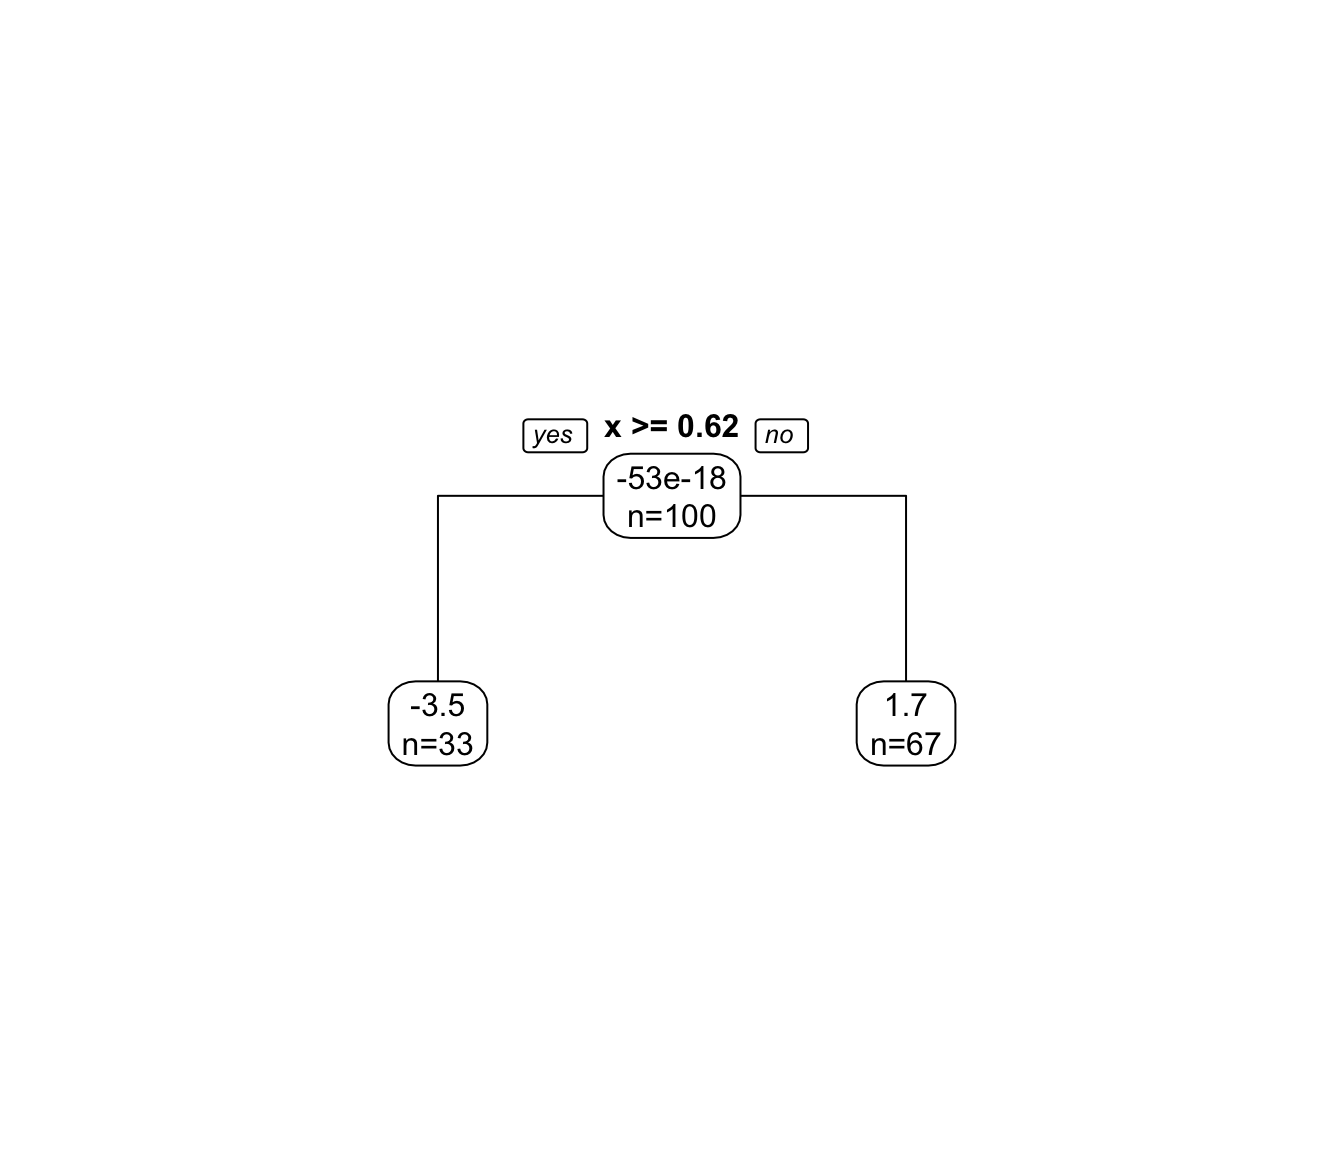
\includegraphics[width=0.7\textwidth,height=\textheight]{boosting_files/figure-pdf/unnamed-chunk-1-2.pdf}

}

\caption{L2 boosting}

\end{figure}%

\begin{figure}[H]

{\centering 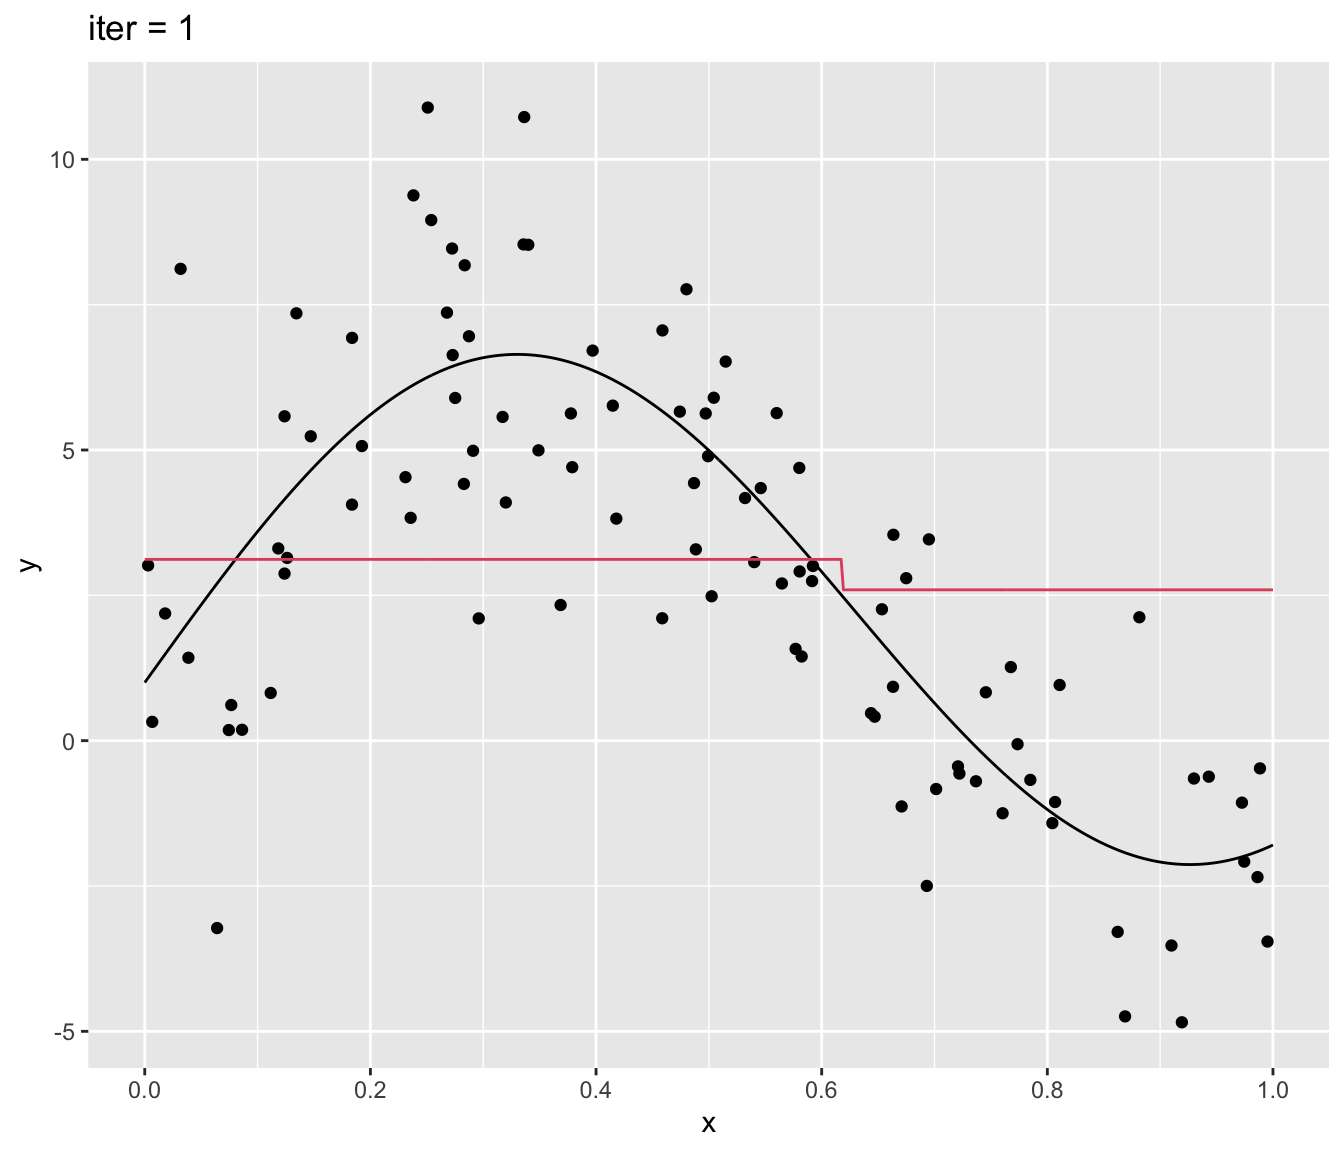
\includegraphics[width=0.7\textwidth,height=\textheight]{boosting_files/figure-pdf/unnamed-chunk-1-3.pdf}

}

\caption{L2 boosting}

\end{figure}%

\subsection{Distributional gradient
boosting}\label{distributional-gradient-boosting}

\begin{itemize}
\tightlist
\item
  \href{https://ar5iv.labs.arxiv.org/html/2204.00778}{Distirbutional
  gradient boosting}
\end{itemize}

\chapter{커널회귀}\label{uxcee4uxb110uxd68cuxadc0}

\section{RKHS}\label{rkhs}

어떤 \(n\times p\) 행렬 \(A\)가 있을 때 이것의 column space를
\(C(A)\)라고 하자.

Ronald Christensen은 아래 \(C(XX^T)=C(X)\)의 결과를 \textbf{the
fundamental theorem of reproducing kernel Hilbert spaces}라고 부른다.

\begin{definition}[Two column spaces are
equiv]\protect\hypertarget{def-equivcs}{}\label{def-equivcs}

For any matrix \(X\), \(C(XX^T)=C(X)\).

\end{definition}

\begin{proof}
Clearly \(C(XX^T)\subset C(X)\), so we need to show that
\(C(X) \subset C(XX^T)\). Let \(x \in C(X)\). Then \(x = Xb\) for some
\(b\). Write \(b=b_0 + b_1\), where \(b_0 \in C(X^T)\) and
\(b1 \perp C(X^T)\). Clearly, \(Xb_1 = 0\), so we have \(x=Xb_0\). But
\(b_0=X^Td\) for some \(d\); so \(x=Xb_0=XX^Td\) and \(x\in C(XX^T)\).
\end{proof}

\begin{definition}[Equivalent Linear
Models]\protect\hypertarget{def-equivlm}{}\label{def-equivlm}

If \(Y=X_1 \beta_1 + e_1\) and \(Y = X_2 \beta_2 +e_2\) are two models
for the same dependent variable vector \(Y\), the models are
\textbf{equivalent} if \(C(X_1) = C(X_2)\).

Since \(C(X) = C(XX^T)\), this implies that the linear models
\(Y= X\beta_1 +e_1\) and \(Y=XX^T\beta_2 +e_2\) are equivalent.

\end{definition}

RKHS는 \(p\)-벡터 \(x_i\)를 \(s\)-벡터 \(\phi_i\)로
\(\phi_i =\begin{bmatrix} \phi_0 (x_i), \cdots \phi_{s-1}(x_i) \end{bmatrix}^T\)로
변환시킨다. \(X\)를 \(x_i^T\)들이 행으로 구성된 행렬로 보면 똑같은
논리로 \(\phi_i^T\)가 행으로 구성된 행렬 \(\Phi\)를 생각할 수 있다.
\(X^X=[x_i^Tx_j]\)를 \(x_i\)들의 inner products로 만드는 \(n\times n\)
행렬로 보면 RKHS는 \textbf{reproducing kernel} \(R(\cdot, \cdot)\)이
존재해 \[
\tilde{R} \equiv [ R(x_i, x_j)]= [\phi_i^T D(\eta) \phi_j] = \Phi D(\eta) \Phi^T
\] 가 \(\phi_i\)들의 \(n\times n\) inner product matrix이며
\(D(\eta)\)가 positive definite diagonal matrix가 됨을 말해준다.
\(D(\eta)\)가 positive definite diagonal matrix이므로 PA책 Theorem
B.22에 의해 \(D(\eta)=QQ^T\)인 정방행렬 \(Q\)가 존재할 것이고 the
fundamental theorem of reproducing kernel Hilbert spaces에 따라 \(s\)가
유한하면 \(C[\Phi D(\eta) \Phi^T] = C(\Phi)\)일 것이다. 따라서 rk 모형
\[
Y = \tilde{R}\gamma + e
\] 를 적합하는 것은 다음의 비모수모형 \[
Y = \Phi \beta + e
\] 를 적합하는 것과 같다. 즉 rk 모형은 \(\beta=D(\eta) \Phi^T \gamma\)로
reparametrization한 것이다. 특별히 rk 모형을 이요해 예측하는 것은 다음과
같이 하면 된다. \[
\hat{y}(x) = \begin{bmatrix} R(x,x_1), \ldots, R(x,x_n) \end{bmatrix} \hat{\gamma}.
\]

\(\Phi\)를 가지고 linear structure를 적합하는 것이나 \(n \times n\) 행렬
\(\tilde{R}\)을 이용해 적합하는 것이나 같을 것이고 이를 \textbf{kernel
trick}이라 한다.

\begin{theorem}[Hilbert space가 RKHS가 되기 위한
조건]\protect\hypertarget{thm-hilbertRKHS}{}\label{thm-hilbertRKHS}

A Hilbert space is a RKHS iff the evaluation functionals are continuous.

\end{theorem}

\section{Kernel Trick}\label{kernel-trick}

Kernel trick의 가장 큰 장점은 알려진 함수 \(R(\cdot, \cdot)\)을 쓰므로
\(\tilde{R}\)을 만들어내기 쉽다는 것이다. 반대로 \(\phi_j (\cdot)\)
함수들에서 \(s\)를 specify하는 것은 시간이 더 걸릴 것이다.

또한 \(n\times s\)행렬 \(\Phi\)는 \(s\)가 크면 이상해지는데,
\(\tilde{R}\)은 항상 \(n\times n\)이 되어 \(s\)가 너무 커질때
이상해지거나 \(s\)가 너무 작을때 단순화되는 것을 막아준다.

\(s\geq n\)이고 \(x_i\)들이 distinct (같은 값을 갖는 \(x\)들이 없다는
뜻)라면 \(\tilde{R}\)은 \(n \times n\) 이고 rank \(n\)인 행렬이며 이것은
saturated model (데이터 수 만큼 모수가 있는 모형)을 만든다. LS
estimate는 fitted value가 obs와 같은 자료를 만들 것이며 d.f는 0이 될
것이다. 즉 overfitting이 있는 것인데, 그래서 보통 kernel trick은
penalized (regularized) estimation과 같이 사용하게 된다.

\(s\geq n\)일 때에는 다른 \(R(\cdot, \cdot)\)을 선택한다 하더라도, 같은
\(C(\tilde{R})\)을 주어 같은 모형을 주는 셈이 된다. 즉 같은 least
squares fits를 준다. 그러나 parametrization을 다르게 하고 거기에
penalty를 주는 방식 (ridge, LASSO 등)으로 다른 fitted value를 만들어낼
수 있다.

사용하려고 하는 \(\phi_j\) 함수들을 다 알고 있을 경우, rk를 쓰는 이득이
었다. 그러나 \(\phi_j\)를 다루기 어렵거나 \(s=\infty\)일 경우에는 rks가
도움이 될 것이다.

다음은 많이 쓰이는 rks들을 정리해 놓았다. \(\|u-v\|\)에만 의존하는
rk들을 \textbf{radial basis function} rk라고 부른다.

\begin{longtable}[]{@{}
  >{\raggedright\arraybackslash}p{(\columnwidth - 2\tabcolsep) * \real{0.5000}}
  >{\raggedright\arraybackslash}p{(\columnwidth - 2\tabcolsep) * \real{0.5000}}@{}}
\toprule\noalign{}
\begin{minipage}[b]{\linewidth}\raggedright
Names
\end{minipage} & \begin{minipage}[b]{\linewidth}\raggedright
\(R(u,v)\)
\end{minipage} \\
\midrule\noalign{}
\endhead
\bottomrule\noalign{}
\endlastfoot
Polynomial of degree \(d\) & \((1+u^Tv)^d\) \\
Polynomial of degree \(d\) & \(b(c+u^Tv)^d\) \\
Gaussian (radial basis) & \(\exp (-b\|u-v\|^2)\) \\
Sigmoid (hyperbolic tangent) & \(\text{tanh}(bu^Tv +c)\) \\
Linear spline (\(u,v\) scalars) & \(\min (u,v)\) \\
Cubic spline (\(u,v\) scalars) &
\(\max (u,v) \min^2 (u,v)/2 - \min^3(u,v)/6\) \\
Thin plate spline (2 dimensions) & \(\|u -v\|^2 \log (\|u - v\|)\) \\
\end{longtable}

표에 있는 것들 중 hyperbolic tangent는 \(\tilde{R}\)을 not nonnegatively
definite한 것들로 줄 수도 있어 실제로 rk는 아니다. 그러나 \(u\)에 대해서
연속인 어떤 \(R(u,v)\)든지 \[
f(x) = \sum_{j=1}^n \gamma_j R(x,x_j)
\] 와 같은 형태의 모형 적합을 유도해낼 수 있기 때문에 이러한 것들을 쓰는
것도 설득력이 있다.

Rk의 아이디어는 함수를 small support를 이용해 근사하는 방법들, 즉
1차원에서 \(s_{*}\)개의 집합으로 나누고 line의 partition을 만들어내는
wavelet, B-spline 등의 방법과 비교할 수 있다. 이러한 방법들은 당연히
\(p\)차원에서 \(s_{*}^p\)개의 dimension을 생각해야 하고 고차원에서
다루기 어렵게 된다. 그러나 kernel method에서는 각 data point에 커널을
적합하는 셈이므로 \(p\)가 크게 커져도 괜찮다.

\section{Kernel Trick과 SVM}\label{kernel-trickuxacfc-svm}

함수 안에 dot product가 있으면 kernel trick을 쓸 수 있다고 한다. 이러한
것들 중 대표적인 것이 SVM이다. SVM의 objective function은 다음과 같다.
\[
\max_{\alpha} \sum_i \alpha_i - \frac{1}{2}\sum_i \sum_j \alpha_i \alpha_j y_i y_j \pmb{x}_i^T\pmb{x}_j ,\quad{} \text{s.t. } \sum_{i} \alpha_i y_i = 0.
\] 이 objective 함수 안에는 dot product \(\pmb{x}_i^T\pmb{x}_j\)가 들어
있고 kernel trick을 쓸 수 있어 SVM이 강력해진다.

\begin{figure}[H]

{\centering 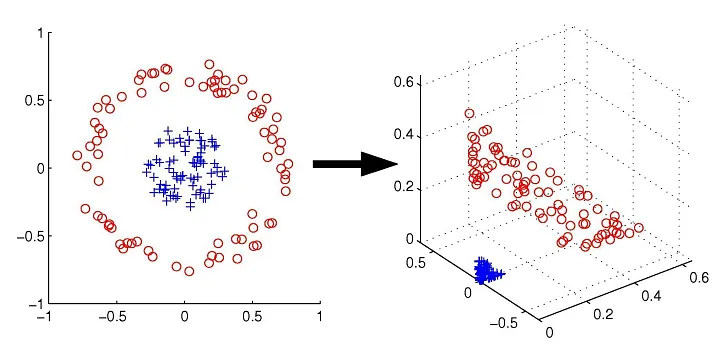
\includegraphics[width=1\textwidth,height=\textheight]{images/kernel_ktrick01.png}

}

\caption{Figure: Example of a labeled data inseparable in 2-Dim is
separable in 3-Dim.}

\end{figure}%

위 그림에서, 원래 자료 \(\pmb{x} = \{x_1, x_2\}\)는 2차원에 있는데
이것은 inseparable 하지만 변환 \[
\Phi (\pmb{x}) \rightarrow (x_1^2, x_2^2, \sqrt{2}x_1x_2)
\] 를 이용해 오른쪽 그림과 같이 바꾸면 분리가능하다.

앞선 \(\Phi\) 변환을 이용했을 때 3D 공간에서 decision boundary는 다음과
같다. \[
\beta_0 + \beta_1 x_1^2 + \beta_2 x_2^2 + \beta_3 \sqrt{2} x_1 x_2 = 0.
\] 만약 로지스틱과 같은 회귀를 이용한다면 위의 식과 같은 모형을 쓸
것이다. 그러나 SVM에서는 kernel trick을 이용해 decision boundary를 만들
수 있다. 이를 위해
\(\langle \Phi(\pmb{x}_i), \Phi(\pmb{x}_j) \rangle\)의 dot product를
찾아야 한다.

\begin{align*}
\langle \Phi(\pmb{x}_i), \Phi(\pmb{x}_j) \rangle &= \langle \{x_{i1}^2, x_{i2}^2, \sqrt{2}x_{i1}x_{i2}\}, \{x_{i1}^2, x_{i2}^2, \sqrt{2}x_{i1}x_{i2}\} \rangle\\
&= x_{i1}^2 + x_{j1}^2 + x_{i2}^2 x_{j2}^2 + 2x_{i1}x_{i2}x_{j1}x_{j2}
\end{align*}

일단 이것을 하려면

\begin{itemize}
\tightlist
\item
  \(\Phi\)를 정의해야 하고
\item
  \(\Phi\) 변환 계산시 \(3\times 2\)의 계산
\item
  그리고 dot product를 계산하는 데 3번 해서
\end{itemize}

총 9번의 계산이 필요하다. 그러나 만약 커널
\(K(\pmb{x}_i,\pmb{x}_j)=\langle \pmb{x}_i,\pmb{x}_j\rangle^2\)을
이용한다면, 변환 \(\Phi\)를 찾을 필요도 없고, 그냥 2차원 공간에서 바로
고차원의 similarity measure (dot product)를 만들어낼 수 있다.

\begin{align*}
\langle \pmb{x}_i,\pmb{x}_j\rangle^2 &= \langle\{ x_{i1}, x_{i2}\},\{ x_{i1}, x_{i2}\} \rangle^2\\
&= (x_{i1}x_{j1} + x_{i2}x_{j2})^2\\
&= x_{i1}^2 + x_{j1}^2 + x_{i2}^2 x_{j2}^2 + 2x_{i1}x_{i2}x_{j1}x_{j2}
\end{align*}

로 만들어낼 수 있다. 이것을 하려면

\begin{itemize}
\tightlist
\item
  \(K\)는 정의해야 하나
\item
  두 번째 식까지 두 번의 operation
\item
  마지막 식에서 제곱을 위해 한 번의 operation
\end{itemize}

3번의 계산이 필요하다.

다른 예제를 보자. Decision boundary를 다음과 같이 정하였다. \[
\beta_0 + \beta_1 x_1 + \beta_2 x_2 + \beta_3 x_1^2 + \beta_4 x_2^2 + \beta_5 \sqrt{2} x_1 x_2 = 0.
\]

\(\Phi(\pmb{x}) \rightarrow (1, \sqrt{2}x_1, \sqrt{2}x_2, x_1^2, x_2^2, \sqrt{2}x_1 x_2)\)와
같이 5차원 변환 \(\Phi\)를 이용해 구하는 방법은 총 16번의 계산을 필요로
한다.

\begin{align*}
\langle \Phi(\pmb{x}_i), \Phi(\pmb{x}_j) \rangle &= \langle \{1, \sqrt{2}x_{i1}, \sqrt{2}x_{i2}, x_{i1}^2, x_{i2}^2, \sqrt{2}x_{i1}x_{i2}\}, \{1, \sqrt{2}x_{i1}, \sqrt{2}x_{i2}, x_{i1}^2, x_{i2}^2, \sqrt{2}x_{i1}x_{i2}\} \rangle\\
&= 1+ 2x_{i1}x_{j1} + 2x_{i2}x_{j2} +x_{i1}^2 x_{j1}^2 + x_{i2}^2 x_{j2}^2 +  x_{i2}^2 x_{j2}^2 + 2x_{i1}x_{i2}x_{j1}x_{j2}
\end{align*}

그러나 커널
\(K(\pmb{x}_i,\pmb{x}_j)=\langle 1+ \langle\pmb{x}_i,\pmb{x}_j\rangle\rangle^2\)를
이용하면 세 번의 계산으로 된다고 한다. \begin{align*}
\langle 1+ \langle\pmb{x}_i,\pmb{x}_j\rangle\rangle^2 &= (1+ x_{i1}x_{j1}+x_{i2}x_{j2})^2\\
&=1+ 2x_{i1}x_{j1} + 2x_{i2}x_{j2} +x_{i1}^2 x_{j1}^2 + x_{i2}^2 x_{j2}^2 +  x_{i2}^2 x_{j2}^2 + 2x_{i1}x_{i2}x_{j1}x_{j2}
\end{align*}

\subsection{무한차원에서의 kernel
trick}\label{uxbb34uxd55cuxcc28uxc6d0uxc5d0uxc11cuxc758-kernel-trick}

앞선 논리를 그대로 적용하면, kernel trick은 infinite space에서도
유사도를 잴 수 있게 해준다. Gaussian Kernel (RBF), exponential kernel,
Laplace kernel 등이 실제로 그러한 역할을 한다. Gaussian kernel은 다음과
같다. \[
K(\pmb{x}_i,\pmb{x}_j)=\exp \Big( - \frac{\| \pmb{x}_i - \pmb{x}_j \|^2}{2\sigma^2} \Big)
\]

\(\sigma=1\)로 두면 위의 Gaussian kernel은
\(C=\exp\Big( -\frac{1}{2}\| \pmb{x}_i\|^2 \Big)\exp\Big( -\frac{1}{2}\| \pmb{x}_j\|^2 \Big)\)으로
두었을 때 \[
\exp \Big( -\frac{1}{2}\| \pmb{x}_i - \pmb{x}_j\|^2 \Big) =C\Big\{ 1- \underbrace{\frac{\langle\pmb{x}_i, \pmb{x}_j \rangle}{1!}}_{\text{1st order}}+\underbrace{\frac{\langle\pmb{x}_i, \pmb{x}_j \rangle^2}{2!}}_{\text{2nd order}}-\underbrace{\frac{\langle\pmb{x}_i, \pmb{x}_j \rangle^3}{3!}}_{\text{3rd order}} + \cdots \Big\}
\] 이러한 표현은 무한차원으로 확장 가능하며, Gaussian kernel이
무한차원에서의 유사도를 찾을 수 있게 해준다.

물론 커널 기반 방법도 커널을 먼저 정해줘야 하며, cross-validation 등을
이용해 커널 함수를 정하거나 또는 커널에 쓰이는 조율모수를 정하게 된다.

\part{Advanced Topics}

\chapter{Robust Regression}\label{robust-regression}

\section{Robust Regression}\label{robust-regression-1}

\begin{itemize}
\tightlist
\item
  \textbf{Robust regression}: 잡음성이 많은 자료에 사용
\end{itemize}

\chapter{Quantile Regression}\label{quantile-regression}

\section{Quantile Regression}\label{quantile-regression-1}

\begin{itemize}
\tightlist
\item
  Check loss function \[
  \rho_\tau (u) = u(\tau - I(u<0))
  \]
\end{itemize}

\begin{figure}[H]

{\centering \includegraphics[width=0.7\textwidth,height=\textheight]{quantreg_files/figure-pdf/unnamed-chunk-1-1.pdf}

}

\caption{Figure: Check loss function.}

\end{figure}%

\chapter{Spatial Linear Models}\label{spatial-linear-models}

\section{Linear Model}\label{linear-model}

\begin{itemize}
\item
  A \textbf{linear model} for a response variable \(Y\) postulates that
  the response is related to the observed values of \(p\) explanatory
  variables \(X_1, \ldots, X_p\) via this equation: \[
  Y = X_1 \beta_1 + X_2 \beta_2 + \cdots + X_p \beta_p + e,
  \] where
\item
  \(\beta_1, \ldots, \beta_p\): (unknown) parameters
  (\textbf{coefficients})
\item
  \(e\): a random variable (\textbf{error})
\item
  \(X_1 \beta_1 + X_2 \beta_2 + \cdots + X_p \beta_p\): mean structure
\item
  When \(n\) obs \((y_1, \pmb{x}_1), \ldots, (y_, \pmb{x}_n)\) are taken
  on the response and explanatory variables, the linear model as just
  defined implied that \[
  y_i = \pmb{x}_i^T \pmb{\beta} + e_i, \quad{} (i=1,\ldots, n)
  \] where
\item
  \(\pmb{\beta} = (\beta_1, \ldots, \beta_p)^T\) and
  \(e_1, \ldots, e_n\) are \(n\) possibly correlated random variables.
\item
  Using vector and matrix notations: \[
  \pmb{y} = \pmb{X \beta} + \pmb{e}.
  \]
\item
  \(\pmb{e}\): \textbf{error vector}
\item
  \(\pmb{\Sigma}\): \(\text{Var}(\pmb{e})\)
\end{itemize}

\section{Spatial Linear Model}\label{spatial-linear-model}

\begin{itemize}
\tightlist
\item
  A \textbf{spatial linear model} is defined as a linear model for
  spatial data for which the elements of \(\pmb{\Sigma}\) are spatially
  structured functions of the data sites
\end{itemize}

\subsection{Spatial Aitken Model}\label{spatial-aitken-model}

\begin{itemize}
\item
  The simplest spatial linear model is an extension of the Gauss-Markov
  model that we call the \textbf{spatial Aitken model}: \[
  \pmb{\Sigma} = \sigma^2 \pmb{R},
  \] where
\item
  \(\sigma^2\): an unknown positive parameter and
\item
  \(\pmb{R}\) is a \textbf{known} positive definite matrix whose
  elements are spatially structured functions of the data sites. We
  refer to \(\pmb{R}\) as the \textbf{scale-free covariance matrix} of
  the observations; in some settings, but not all, it is a correlation
  matrix.
\item
  Estimation: \textbf{generalized least squares (GLS)}
\end{itemize}

\begin{example}[A toy example of a spatial Aitken
model]\protect\hypertarget{exm-Aitken}{}\label{exm-Aitken}

Consider four obs located at the corners of the unit square in
\(\mathbb{R}^2\), ordered such that the first and last obs are located
at opposite corners of the square. Suppose that the model for the obs is
given by \[
\pmb{R} = 
\begin{pmatrix}
1 & e^{-1} & e^{-1} & e^{-\sqrt{2}}\\
e^{-1} & 1 & e^{-\sqrt{2}} & e^{-1}\\
e^{-1} & e^{-\sqrt{2}} & 1 & e^{-1}\\
e^{-\sqrt{2}} & e^{-1} & e^{-1} & 1
\end{pmatrix}
\]

\end{example}

\begin{itemize}
\item
  \textbf{Symmetric}
\item
  \textbf{Positive definiteness}: the variance of any linear
  combinations of obs having this cov matrix, expect the trivial linear
  combination with all coeffs equal to zero.
\end{itemize}

\section{Spatial General Linear
Model}\label{spatial-general-linear-model}

\begin{itemize}
\item
  A more flexible spatial linear model
\item
  \(\pmb{\Sigma}\) is not fully specified but is given by a
  \textbf{known} spatially structured, matrix-valued parametric function
  \(\pmb{\Sigma}(\pmb{\theta})\), where \(\pmb{\theta}\) is an
  \textbf{unknown} parameter vector.
\item
  Joint parameter space for \(\pmb{\beta}\) and \(\pmb{\theta}\)
  generally taken to be \[
  \{ (\pmb{\beta}, \pmb{\theta}): \pmb{\beta} \in \mathbb{R}^p, \pmb{\theta} \in \Theta \subset \mathbb{R}^m \}
  \] where
\item
  \(\Theta\): the set of vectors \(\pmb{\theta}\) for which
  \(\pmb{\Sigma}(\pmb{\theta})\) is symmetric and positive definite, or
  possibly some subset of that set.
\end{itemize}

\begin{refremark}
A spatial Aitken model is a special case of a spatial general linear
model, with \(\pmb{\theta} \equiv \sigma^2\) and \(\pmb{R}\) not
functionally dependent on any unknown parameters.

\label{rem-Aitken}

\end{refremark}

\begin{example}[A toy example of a spatial Aitken model
(2)]\protect\hypertarget{exm-Aitken2}{}\label{exm-Aitken2}

\[
\pmb{\Sigma}(\pmb{\theta}) = \sigma^2
\begin{pmatrix}
1 & e^{-1/\alpha} & e^{-1/\alpha} & e^{-\sqrt{2}/\alpha}\\
e^{-1/\alpha} & 1 & e^{-\sqrt{2}/\alpha} & e^{-1/\alpha}\\
e^{-1/\alpha} & e^{-\sqrt{2}/\alpha} & 1 & e^{-1/\alpha}\\
e^{-\sqrt{2}/\alpha} & e^{-1/\alpha} & e^{-1/\alpha} & 1
\end{pmatrix}
\]

The parameter space for \(\pmb{\theta} \equiv (\sigma^2, \alpha)^T\)
within which \(\pmb{\Sigma}(\pmb{\theta})\) is p.d. is \[
\{ (\sigma^2, \alpha) : \sigma^2 > 0 , \alpha >0 \}
\]

Small values of \(\alpha\) correspond to weak spatial correlation among
the obs, and as \(\alpha\) increases the spatial correlation among obs
become stronger.

\end{example}

\chapter{Gaussian Processes}\label{gaussian-processes}

\section{Regression analysis}\label{regression-analysis-1}

\begin{itemize}
\item
  All finite collection of realizations (\(n\) obs) is modeled as having
  a multivariate normal (MVN) distribution.
\item
  \textbf{Mean function}: \(\mu (x)\)
\item
  \textbf{Covariance function}: \(\Sigma (x, x')\)
\item
  \(\Sigma (x, x') = \exp \{ - \| x- x' \|^2 \}\)
\item
  \(\Sigma (x, x )=1\)
\item
  \(\Sigma (x, x')\) must be \textbf{positive definite}
\item
  \(\Sigma_n\): covariance matrix (p.d.)
\end{itemize}

\section{Splines vs GP}\label{splines-vs-gp}

\chapter{PCA and Least Squares}\label{pca-and-least-squares}

\section{PCA as least squares
problems}\label{pca-as-least-squares-problems}

PCA can be formulated as follows:

Given \(m\) vectors \(\pmb{x}_1, \ldots, \pmb{x}_m \in \mathbb{R}^n\),
find matrices \(\pmb{U} \in \mathcal{M}_{\mathbb{R}} (k,n)\) and
\(\pmb{V} \in \mathcal{M}_{\mathbb{R}}(n,k)\) such that \[
\sum_{i=1}^m \| \pmb{x}_i - \pmb{V}\pmb{U}\pmb{x}_i\|^2
\] is minimized.

That is, for \(k<n\), the vector \(\pmb{U}\pmb{x}_i \in \mathbb{R}^k\)
is the projection of \(\pmb{x}_i\) into a lower-dimensional subspace,
and \(\pmb{V}\pmb{U}\pmb{x}_i\) is the \textbf{reconstructed} original
vector. PCA aims to find matrices \(\pmb{U}\), \(\pmb{V}\) that minimize
the reconstruction error as measured by the \(\ell^2\)-norm. It can be
shown that, in fact, these matrices are orthogonal and
\(\pmb{U} = \pmb{V}^T\), so the problem reduces to \[
\arg\min_{V\in \mathcal{M}_{\mathbb{R}}(n,k)}\sum_{i=1}^m \| \pmb{x}_i - \pmb{V}\pmb{V}^T \pmb{x}_i \|^2
\] Further manipulations show that \(\pmb{V}\) is the matrix whose
columns are the eigenvectors corresponding to the \(k\) largest
eigenvalues of \[
\sum_{i=1}^m \pmb{x}_i \pmb{x}_i^T
\] as expected. So indeed, PCA is a least squares method and it is quite
sensitive to outliers.

\bookmarksetup{startatroot}

\chapter{Summary}\label{summary}

In summary, this book has no content whatsoever.

\begin{Shaded}
\begin{Highlighting}[]
\DecValTok{1} \SpecialCharTok{+} \DecValTok{1}
\end{Highlighting}
\end{Shaded}

\begin{verbatim}
[1] 2
\end{verbatim}

\bookmarksetup{startatroot}

\chapter*{References}\label{references}
\addcontentsline{toc}{chapter}{References}

\markboth{References}{References}

\phantomsection\label{refs}
\begin{CSLReferences}{1}{0}
\bibitem[\citeproctext]{ref-Hansen2022}
Hansen, Bruce. 2022. \emph{Econometrics}. Princeton University Press.

\end{CSLReferences}



\end{document}
